Evaluation of ESN performance on the NARMA system is a thoroughly explored area
in the field of RC \cite{verstraeten_experimental_2007, rodan_minimum_2011,
jaeger_adaptive_nodate}. Similar performance to previous work has been achieved
(Fig. \ref{performance}) lending credibility to further approaches in this
paper.

\begin{figure}[H]
  \centering
  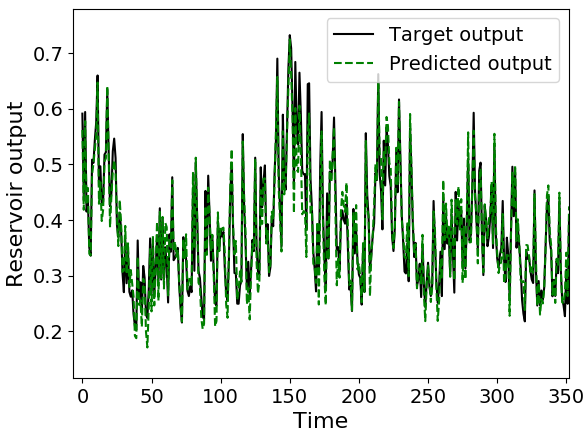
\includegraphics[width=2.5in]{img/narma_visualization.png}
  \caption{
    Visualization of reservoir output. (TODO): Re-do this screenshot so it's
possible to see anything at all.
  }
  \label{visualization}
\end{figure}

\begin{figure}[H]
  \centering
  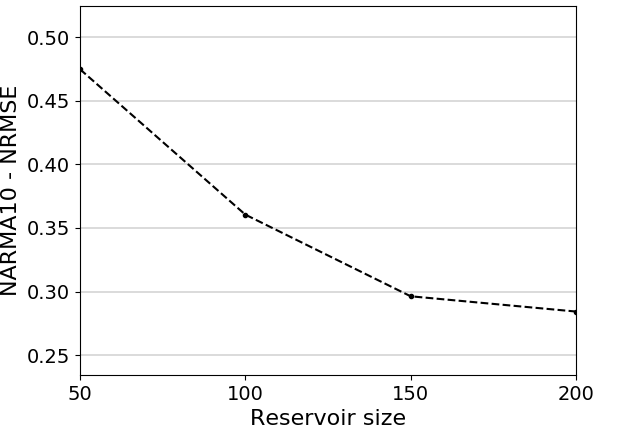
\includegraphics[width=2.5in]{img/general_performance.png}
  \caption{
    ESN performance. Performed with input scaling of 1, spectral radius 0.9,
input sparsity of 1.0, no leaky nodes. 10 random reservoirs were sampled for
each reservoir size.
  }
  \label{performance}
\end{figure}
% (TODO): Fix caption to suck less for both of these^.

\subsection{Noise}

\subsection{Measurement equipment accuracy}

\subsection{Partial visible state}

\subsection{Topology}


% Thoughts
% * Remember to add NRMSE to heatmap plots.

%%% Local Variables:
%%% mode: latex
%%% TeX-master: "../main"
%%% End:
